\subsection{Evolutionäre Algorithmen}
Bei der Implementierung der Evolutionären Ansätze wurde insbesondere Wert darauf gelegt, dass sowohl die theoretischen Grundlagen abgebildet sind als auch dass die verschiedenen Ansätze mit der grundsätzlich selben Struktur implementiert werden können um Redundanz im Code so gut als möglich zu vermeiden. Mit diesen Zielen vor Augen wurde folgende Grundstruktur für die Implementierung von evolutionären Algorithmen entworfen:

\begin{figure}[h]
  \centering
  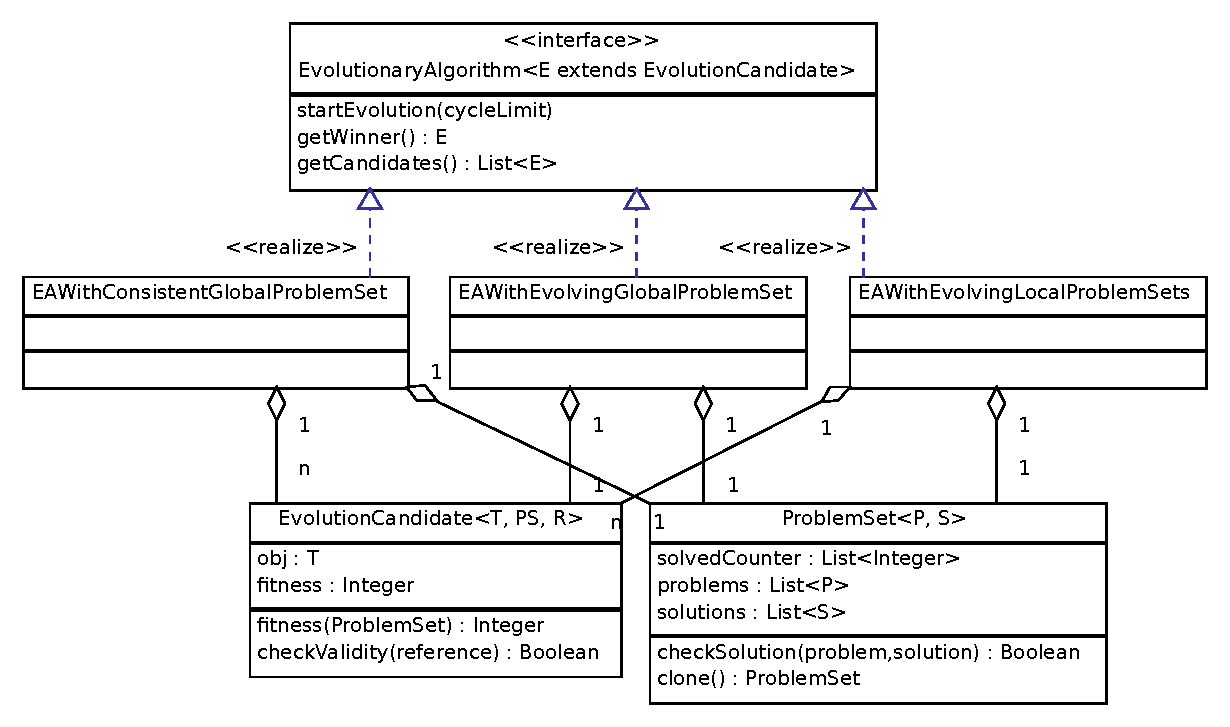
\includegraphics[width=0.8\textwidth]{images/simple_uml_evolution.pdf}
  \caption[EA Grundstruktur Klassendiagramm]{EA Grundstruktur vereinfacht}
  \label{fig:ea_classdiag_simple}
\end{figure}

Die Klassen welche die Algorithmen beinhalten verwenden eine Menge von \lstinline$EvolutionCandidate$ (Population) und ein \lstinline$ProblemSet$. Der evolutionäre Algorithmus kann jeweils mit \lstinline$startEvolution$ gestartet werden und wird abgebrochen sobald eine gültige Lösung gefunden wurde.

Das \lstinline$ProblemSet$ besteht Grundsätzlich aus zwei Listen. In der Ersten ist die \flqq Problemstellung\frqq abgelegt, in der zweiten die entsprechenden Musterlösung. Mithilfe der Methode \lstinline$checkSolution(problem, solution)$ kann geprüft werden ob eine erarbeite Lösung (Parameter \lstinline$solution$) der Musterlösung entspricht. In unserem Fall wird so geprüft, ob unser Automat die Zugehörigkeit eines Wortes zu der gegebenen Sprache richtig erkennt oder nicht.

Der \lstinline$EvolutionCandidate$ entspricht einem Individuum aus unserer Population und besteht aus dem \flqq obj\frqq, welches in unserem Fall den Automaten an sich beinhaltet, der \lstinline$fitness$ als Eigenschaft (wird zur Sortierung verwendet) und einer \lstinline$fitness$ Funktion welche ein \lstinline$ProblemSet$ entgegen nimmt und mithilfe des gegebenen \flqq obj\frqq versucht alle Probleme aus dem \lstinline$ProblemSet$ zu lösen. Die Fitness als Wert entspricht der Anzahl korrekt gelöster Probleme.

\subsubsection{Initialisierung}
Um die Klassen der evolutionären Algorithmen schlank zu halten, wurde die Initialisierung ausgelagert. In der Abbildung \ref{fig:ea_init_classdiag_simple} sieht man, dass die Initialisierung eines evolutionären Algorithmus zur Findung eines endlichen Automaten zu einem gegebenen regulären Ausdruck in drei Schritten abläuft:
\begin{enumerate}
	\item Sprache initialisieren (\lstinline$initLanguage(alphabet, maxWordLength, regexp)$)
	\item Probleme initialisieren (\lstinline$initProblems(noProblems)$)
	\item Population initialisieren (\lstinline$initCandidates(noCandidates)$)
\end{enumerate}

\begin{figure}[h]
  \centering
  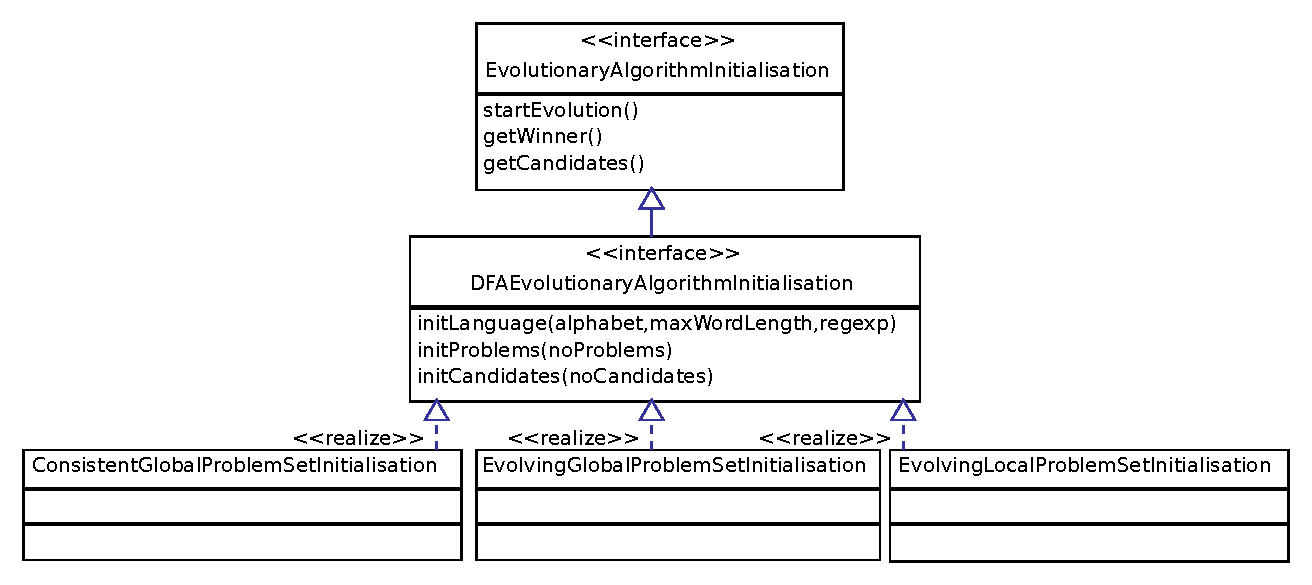
\includegraphics[width=0.8\textwidth]{images/simple_uml_evolution_initialisation.pdf}
  \caption[EA Initialisierung Klassendiagramm]{EA Initialisierung Klassendiagramm}
  \label{fig:ea_init_classdiag_simple}
\end{figure}

\paragraph{Initialisierung der Sprache}
Beim initialisieren der Sprache werden das Alphabet und der reguläre Ausdruck für die spätere Verwendung abgelegt, es wird eine Instanz des \lstinline$WordProblemGenerator$s angelegt und ein Referenzautomat (\lstinline$dk.brics.automaton$) wird erzeugt, welcher später zur Überprüfung von Resultaten verwendet wird.

\paragraph{Generieren von Problemen}
Probleme werden von einem \lstinline$ProblemGenerator$ erzeugt. Die für dieses Problem erstellte Implementation \lstinline$WordProblemGenerator$ generiert mithilfe eines gegebenen Alphabets Tupel vom Typ \lstinline$Tuple<CharArray, Boolean>$ wobei im \lstinline$CharArray$ eine zufällige Zeichenfolge der Zeichen aus dem Alphabet mit einer zufälligen länge zwischen 0 und \lstinline$maxWordLength$ Zeichen ist. Der Boolean zeigt an, ob die generierte Zeichenfolge vom ebenfalls gegebenen \lstinline$regexp$ akzeptiert wird oder nicht.

Zu dem generieren von einzelnen \flqq Problem\frqq - \flqq Lösung\frqq Tupeln kann der Problemgenerator auch ganze ProblemSets generieren. Als Parameter hierfür benötigt der \lstinline$WordProblemGenerator$ die gewünschte Länge des Sets und ein Flag welches angibt ob der leere String immer im Set vorhanden sein soll oder nicht.

\begin{figure}[h]
  \centering
  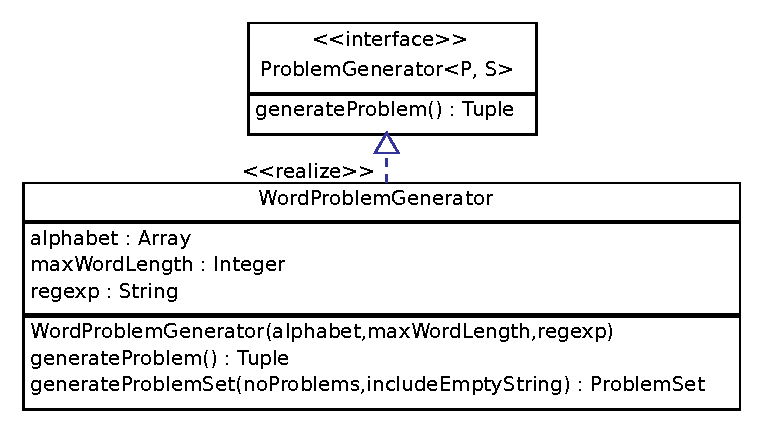
\includegraphics[width=0.5\textwidth]{images/simple_uml_pg.pdf}
  \caption[Problemgenerierung Klassendiagramm]{Problemgenerierung Klassendiagramm}
  \label{fig:ea_pg_classdiag_simple}
\end{figure}


\paragraph{Generieren von Lösungskandidaten}
Das Generieren von zufälligen Automaten mit einem gegebenen Alphabet erledigt der Konstruktor der \lstinline$RandomDeterministicFiniteAutomaton$ Klasse. Eine detaillierte Beschreibung wie die Automaten zufällig zusammengestellt werden befindet sich im Kapitel \ref{subsec:RandomDeterministicFiniteAutomaton}.
